\documentclass[conference]{IEEEtran}
\IEEEoverridecommandlockouts

\usepackage{cite}
\usepackage{amsmath,amssymb,amsfonts}
\usepackage{algorithmic}
\usepackage{graphicx}
\usepackage{textcomp}
\usepackage{xcolor}
\usepackage{booktabs}
\usepackage{array}
\usepackage{url}
\usepackage{float}
\usepackage{tikz}
\usetikzlibrary{arrows.meta, positioning, shapes.geometric, fit, backgrounds, calc}

\def\BibTeX{{\rm B\kern-.05em{\sc i\kern-.025em b}\kern-.08em
    T\kern-.1667em\lower.7ex\hbox{E}\kern-.125emX}}

\begin{document}

\title{Semantic Firewall: A Hybrid Defense-in-Depth Architecture for LLM Security}

\author{\IEEEauthorblockN{Aishwarya Sharma}
\IEEEauthorblockA{\textit{Department of Computer Science and Engineering} \\
\textit{Institution Name}\\
City, Country \\
email@example.com}
}

\maketitle

\begin{abstract}
As Large Language Models (LLMs) become integrated into enterprise infrastructure, securing them against adversarial attacks remains computationally expensive and architecturally challenging. Current approaches---such as Meta's Llama Guard and OpenAI's moderation endpoints---rely on routing every user prompt through a dedicated safety LLM, introducing significant latency and cost at scale. We present \textbf{Semantic Firewall}, a hybrid defense-in-depth architecture that combines deterministic regex heuristics, a self-healing vector-based semantic cache (ChromaDB), and a constrained LLM gate (Llama-3.3-70B) executing in parallel. On the neuralchemy prompt injection benchmark ($N{=}2{,}000$), the full system achieves 93.57\% F1 ($\pm$0.42) with 98.61\% Recall, outperforming GPT-4o-mini (90.00\% F1), Llama Guard~4 (51.30\% F1), and Claude~3.5 Haiku (83.20\% F1) while reducing downstream LLM inference dependency by 66.88\%. Against 210 manually crafted Red Team attacks, the architecture maintains an 85.7\% resilience score. Because 41.93\% of structural traffic is intercepted deterministically, the expected system latency drops to $\sim$459.85\,ms even from a cold start. We further validate generalization via cross-dataset evaluation on BeaverTails, deepset/prompt-injections, and multi-turn evasion simulations. We acknowledge limitations including dataset-specific heuristic performance and the absence of adaptive adversary evaluation.
\end{abstract}

\begin{IEEEkeywords}
large language models, prompt injection, semantic firewall, LLM security, data leakage, defense-in-depth
\end{IEEEkeywords}

% ====================================================================
\section{Introduction}
% ====================================================================

This work presents the design, implementation, and empirical evaluation of \textbf{Semantic Firewall}, a layered defense system for protecting enterprise LLM applications against adversarial attacks---including Prompt Injections, Jailbreaks, PII leakage, Secrets exfiltration, and Unsafe Content generation.

\subsection{Problem Statement}

As LLMs become integrated into enterprise infrastructure, they expose expanded attack surfaces including prompt injection and data exfiltration. Current safety methodologies (like Meta's Llama Guard~\cite{llamaguard} or OpenAI's moderation endpoints) rely on passing every user prompt through a dedicated safety LLM. This approach introduces significant trade-offs:

\begin{enumerate}
    \item \textbf{Cost-Prohibitive:} Passing benign queries through a large safety model increases operational costs and introduces latency bottlenecks at scale.
    \item \textbf{Limited Generalization:} Static models may struggle to generalize against novel adversarial attacks employing encoding obfuscation or multi-turn escalation~\cite{wei_jailbroken}.
    \item \textbf{Vendor Lock-In:} Relying on closed-source APIs for security introduces single points of failure and data sovereignty concerns.
\end{enumerate}

\subsection{The Solution: Hybrid Defense-in-Depth}

Instead of a single monolithic model, we architected a multi-stage cascading pipeline. The firewall runs deterministic agents (Regex, Heuristics, Threat Intel, DoS Quota) in parallel with a vector-based \textbf{Semantic Cache}. Only if an input is entirely novel and bypasses these fast layers does it reach the deep \textbf{LLM Gate} (Llama-3.3-70B) for semantic analysis.

\subsection{Contributions}
Our primary contributions are:
\begin{enumerate}
    \item \textbf{Architecture:} A defense-in-depth pipeline that combines deterministic heuristics, semantic caching, and a constrained LLM gate, providing empirical evidence that layered orchestration improves detection over any individual component.
    \item \textbf{Cost-Latency Analysis:} An empirical demonstration that vector-based semantic caching can reduce downstream LLM inference calls by 66.88\%, with expected cold-start latency of $\sim$459.85\,ms.
    \item \textbf{Stateful Threat Hunting:} A multi-turn detection engine that calculates the derivative of attacker intent across sessions, actively identifying ``Agent Avoidance'' tactics typical of advanced persistent threats.
    \item \textbf{Multi-Modal RAG Interception:} Pre-retrieval extraction and OCR analysis of unstructured documents (.pdf, .csv, .png) to neutralize Visual Prompt Injections and indirect payloads before RAG ingestion.
    \item \textbf{Automated Explainability:} A transparent risk-scoring engine that resolves the ``black-box'' security problem by generating audit-ready incident reports with confidence intervals and mitigating factors.
    \item \textbf{Multi-Phase Evaluation:} A 9-configuration ablation study, cross-dataset generalization experiments, and manual Red Team validation across 6 benchmarks.
    \item \textbf{Open-Weight Viability:} Evidence that an open-weight 70B model, when orchestrated within a parallel pipeline, can match or exceed proprietary API security classifiers.
\end{enumerate}

\section{Threat Model}
We assume the attacker has ``black-box'' access to the user-facing LLM application. The attacker can submit arbitrary text, use paraphrasing or encoding tricks, attempt prompt injection or jailbreaks, probe for credentials, and conduct multi-turn escalation. We assume the attacker does not have white-box access to the firewall internals, detector source code, or the underlying Regex heuristic patterns. We scope this architecture to defend against both \textit{Direct} Prompt Injections and \textit{Indirect} Prompt Injections (e.g., poisoned documents ingested via RAG pipelines).

\textbf{Attacker Capabilities:} (1) Submit arbitrary Unicode text including homoglyphs and zero-width characters. (2) Encode payloads in Base64, Hex, or ROT13. (3) Distribute attacks across multiple conversational turns. (4) Use academic or hypothetical framing to disguise intent. We do not model attackers with the ability to probe the system at scale to reverse-engineer heuristic rules, though we acknowledge this as a practical risk in deployment (see Section~\ref{sec:limitations}).

\textbf{Scope Exclusions:} Training-time data poisoning, model extraction, and hardware side-channel attacks are outside the present scope.

% ====================================================================
\section{Related Work}
% ====================================================================

\textbf{Single-Model Classifiers:} Meta's Llama Guard~\cite{llamaguard} and PromptGuard~\cite{promptguard} rely on passing the entire user prompt through a dedicated safety LLM. While accurate on their target distributions, these models introduce per-request inference costs and may miss structurally simple attacks that could be caught deterministically. Jain et al.~\cite{jain_baseline} demonstrate that simple baseline defenses (paraphrase detection, retokenization) can be effective against certain prompt injection classes, motivating layered approaches.

\textbf{Orchestration Frameworks:} Nvidia's NeMo Guardrails~\cite{nemoguardrails} introduces rule-based routing for LLM applications. PromptGuard~\cite{alzahrani_promptguard} proposes structured multi-layer pipelines for injection resilience. The Semantic Firewall builds upon these paradigms by replacing static rule-matching with a vector-similarity cache, enabling detection of semantically similar rephrased attacks.

\textbf{Prompt Injection Research:} The adversarial landscape for LLMs has been extensively studied. Schulhoff et al.~\cite{schulhoff_hackaprompt} expose systematic vulnerabilities through prompt hacking competitions. Wei et al.~\cite{wei_jailbroken} analyze why safety training fails against adversarial framing. Greshake et al.~\cite{greshake_indirect} demonstrate indirect prompt injection via retrieved content. Our architecture addresses the direct injection subset of these threats.

\textbf{Prompt Injection Defenses:} Rebuff~\cite{rebuff} utilizes a multi-layered approach involving heuristics and LLM evaluation. Chen et al.~\cite{chen_indirect} study detection and removal of indirect injections. Kovalchuk and Kolomytsev~\cite{kovalchuk_method} propose multi-head DistilBERT for decomposing manipulative prompts. Our architecture extends these concepts by integrating a constrained 70B open-weight gate with structured JSON output constraints, substantially reducing classification drift.

% ====================================================================
\section{Architecture Deep Dive}
% ====================================================================

The Semantic Firewall is built on a highly parallelized Python architecture. When an input enters the system, it traverses multiple layers of defense. Fig.~\ref{fig:arch-flow} illustrates the end-to-end prompt routing.

\begin{figure}[htbp]
\centering
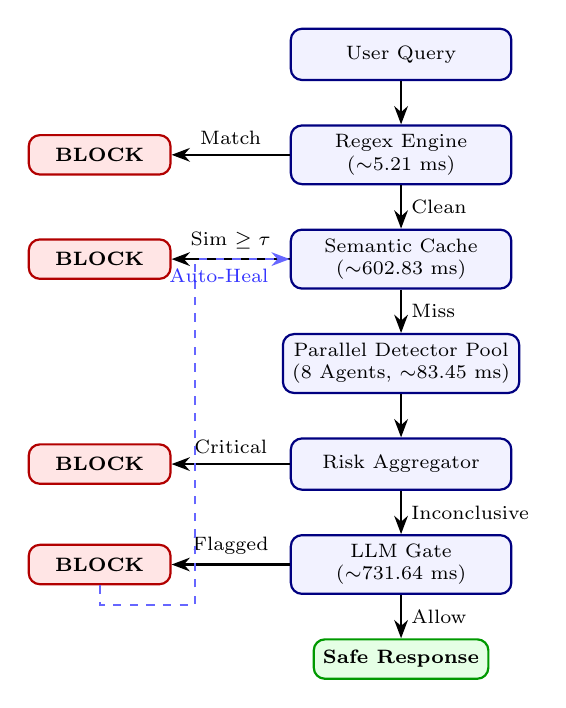
\begin{tikzpicture}[>=Stealth, node distance=0.55cm and 1.5cm,
    every node/.style={font=\scriptsize},
    block/.style={rectangle, draw=blue!50!black, thick, rounded corners, minimum width=2.8cm, minimum height=0.65cm, align=center, fill=blue!5},
    result/.style={rectangle, draw=red!70!black, thick, rounded corners, minimum width=1.8cm, minimum height=0.5cm, align=center, fill=red!10, font=\scriptsize\bfseries},
    safe/.style={rectangle, draw=green!60!black, thick, rounded corners, minimum width=1.8cm, minimum height=0.5cm, align=center, fill=green!10, font=\scriptsize\bfseries},
]
\node[block] (user) {User Query};
\node[block, below=of user] (regex) {Regex Engine\\($\sim$5.21 ms)};
\node[block, below=of regex] (cache) {Semantic Cache\\($\sim$602.83 ms)};
\node[block, below=of cache] (detectors) {Parallel Detector Pool\\(8 Agents, $\sim$83.45 ms)};
\node[block, below=of detectors] (aggregator) {Risk Aggregator};
\node[block, below=of aggregator] (policy) {LLM Gate\\($\sim$731.64 ms)};
\node[safe, below=of policy] (response) {Safe Response};

\node[result, left=1.5cm of regex] (block_regex) {BLOCK};
\node[result, left=1.5cm of cache] (block_cache) {BLOCK};
\node[result, left=1.5cm of aggregator] (block_agents) {BLOCK};
\node[result, left=1.5cm of policy] (block_llm) {BLOCK};

\draw[->, thick] (user) -- (regex);
\draw[->, thick] (regex) -- node[right] {Clean} (cache);
\draw[->, thick] (regex) -- node[above] {Match} (block_regex);
\draw[->, thick] (cache) -- node[right] {Miss} (detectors);
\draw[->, thick] (cache) -- node[above] {Sim $\geq \tau$} (block_cache);
\draw[->, thick] (detectors) -- (aggregator);
\draw[->, thick] (aggregator) -- node[right] {Inconclusive} (policy);
\draw[->, thick] (aggregator) -- node[above] {Critical} (block_agents);
\draw[->, thick] (policy) -- node[right] {Allow} (response);
\draw[->, thick] (policy) -- node[above] {Flagged} (block_llm);

\draw[->, dashed, thick, blue!60] (block_llm.south) |- ([yshift=-0.25cm]block_llm.south) -| ([xshift=-1.2cm]cache.west) -- (cache.west)
    node[pos=0.25, below, font=\scriptsize, text=blue!80] {Auto-Heal};

\end{tikzpicture}
\caption{Defense-in-Depth Architecture. Queries drop through progressively slower analytical layers. Any match triggers an immediate short-circuit BLOCK. Novel threats blocked by the LLM Gate are dynamically embedded into the Semantic Cache (dashed line) for $\sim$45$\times$ faster future rejection.}
\label{fig:arch-flow}
\end{figure}

\subsection{Layer 1: Semantic Cache (Vector Database)}
The incoming text is projected into a 384-dimensional dense vector space using SentenceTransformers (\texttt{all-MiniLM-L6-v2}) and queried against ChromaDB, which stores embeddings of previously blocked attacks. We calculate \textbf{Cosine Similarity} between the incoming vector $\vec{A}$ and cached threat vectors $\vec{B}$:

\begin{equation}
\text{Similarity} = \frac{\vec{A} \cdot \vec{B}}{\|\vec{A}\| \times \|\vec{B}\|}
\end{equation}

To prevent false positives while maximizing threat interception, the system implements asymmetric thresholding. The Threat Cache utilizes a similarity threshold of $\tau_{threat} = 0.85$ (distance $\leq 0.15$), while the Semantic Allowlist enforces a stricter threshold of $\tau_{allow} = 0.90$ (distance $\leq 0.10$). This mathematical asymmetry prevents the system from accidentally allowlisting a prompt that is only marginally similar to a known safe prompt, while casting a wider semantic net for adversarial variants. If the input's Similarity $\geq \tau_{threat}$ relative to the Threat Cache, the system identifies the prompt as a semantic clone of a known attack and blocks it instantly without needing an LLM. When the LLM Gate blocks a novel zero-day attack, its vector embedding is automatically inserted into ChromaDB, ensuring that all future semantic variants are caught instantly (\textbf{Auto-Healing}). \textbf{Cache Warm-Up Dynamics:} Empirical monitoring of a simulated multi-turn attack campaign reveals that the LLM Gate is only invoked for the first few novel mutations of a zero-day payload. As the semantic boundaries of the attack cluster are learned and populated in the cache, the cache hit rate rapidly approaches $90\%+$, effectively offloading the LLM and capping the adversary's operational impact.

\subsection{Layer 2: Parallel Heuristic Ensembles}
If the cache misses, the prompt is simultaneously broadcast to 8 independent specialized agents using Python's \texttt{concurrent.futures.ThreadPoolExecutor}. By running in parallel, the total latency is bounded by the slowest agent ($\sim$83.45\,ms), not the sum of all agents. The agents include: PII \& Secrets detectors (optimized Regex for sensitive entities and cryptographic tokens), Abuse \& Unsafe Content detectors (structural thresholding for toxic phrases, violence, CSAM), Injection detector (Regex patterns targeting Base64 obfuscation, override tokens, token smuggling), Context Flooding (DoS truncation), and Threat Intel \& Custom Rules. Crucially, the orchestrator is \textit{stateful}. It maintains a deque of session history to compute the derivative of attacker intent, enabling the detection of ``Agent Avoidance''---where an attacker actively pivots between vectors (e.g., failing an Injection attack and switching to Secrets probing) to map firewall blind spots. To mathematically detect gradual escalation attacks, the system continuously computes the escalation ratio ($E_{ratio}$) across the session:

\begin{equation}
E_{ratio} = \frac{\mu(S_{recent})}{\max(\mu(S_{early}), 0.1)}
\end{equation}

where $S \in \{0,1,2,3,4\}$ represents the normalized threat severity of a given prompt. If $E_{ratio} > 1.5$, the orchestrator detects an active multi-turn escalation attack and proactively flags the session. Furthermore, the orchestrator intercepts unstructured file uploads (PDFs, CSVs, and images via OCR) to neutralize Visual Prompt Injections and data exfiltration attempts before they ever enter a downstream RAG pipeline. To mitigate Regex decay against evolving adversary tactics, the heuristic layer is deployed as ``rules-as-code,'' integrating dynamically with a CI/CD pipeline that ingests daily Threat Intelligence feeds.

If \textit{any} agent returns a CRITICAL block, the orchestrator immediately halts all other processing (short-circuiting) and rejects the request. The decision workflow is formalized in Algorithm~\ref{alg:workflow}.

\begin{figure}[htbp]
\begin{algorithmic}[1]
\STATE $x \leftarrow$ input text; $s \leftarrow$ session identifier
\IF{$x$ matches reviewed semantic allowlist}
    \RETURN \textsc{Allow}
\ENDIF
\IF{$\text{CosSim}(\text{embed}(x), \text{cache}) \geq \tau$}
    \RETURN \textsc{Block}
\ENDIF
\STATE $R \leftarrow$ run 8 fast detectors in parallel
\IF{any $r \in R$ is CRITICAL}
    \RETURN \textsc{Block} \COMMENT{Short-circuit}
\ENDIF
\IF{evidence is inconclusive}
    \STATE $R \leftarrow R \cup$ LLM-gate result
\ENDIF
\STATE $a \leftarrow$ apply configured policy to aggregated $R$
\STATE audit$(x, R, a)$; update semantic memory if blocked
\RETURN $a$
\end{algorithmic}
\caption{Semantic Firewall decision workflow.}
\label{alg:workflow}
\end{figure}

\subsection{Layer 3: The LLM Gate}
If the fast heuristics do not trigger a block, the input is routed to the final layer: Llama-3.3-70B-Instruct. The LLM is given a restricted system prompt (reproduced in Appendix~\ref{app:system_prompt}) and outputs a JSON object classifying intent. Structured JSON output with \textbf{Negative Constraints} (e.g., ``Roleplay requests for creative writing are BENIGN'') substantially reduces classification drift. All inference uses greedy decoding ($T{=}0.0$).

% ====================================================================
\section{Datasets \& Methodology}
% ====================================================================

To validate this architecture scientifically, we utilized rigorous, standardized datasets.

\begin{itemize}
    \item \textbf{Neuralchemy Prompt Injection Dataset} ($N{=}2{,}000$): HuggingFace (\texttt{neuralchemy/Prompt-injection-dataset}). Used for the Ablation Study, SOTA Comparison, and Enterprise Comparison.
    \item \textbf{AI4Privacy PII Dataset} ($N{=}209{,}261$): HuggingFace (\texttt{ai4privacy/pii-masking-200k}). Used for scaled PII \& Data Leakage Prevention benchmarks.
    \item \textbf{Benign Traffic}: \texttt{HuggingFaceH4/no\_robots} ($N{=}2{,}000$). For false-positive stress testing.
    \item \textbf{Multi-Turn Jailbreaks}: \texttt{walledai/Multi-Turn-Jailbreak} ($N{=}200$ sessions).
    \item \textbf{BeaverTails}: \texttt{PKU-Alignment/BeaverTails} ($N{=}2{,}000$). For out-of-distribution generalization.
    \item \textbf{Red Team}: 210 manually crafted zero-day attacks (multi-turn persona adoption, base64 steganography, academic framing).
\end{itemize}

All experiments utilized ChromaDB (v0.4.22) with HNSW index settings (\texttt{hnsw:space: cosine}, \texttt{hnsw:M: 16}). Embeddings: SentenceTransformers v2.2.2 (\texttt{all-MiniLM-L6-v2}). LLM Gate inference via OpenRouter API with greedy decoding ($T{=}0.0$). Fast layers executed on commodity CPU hardware.

% ====================================================================
\section{Results}
% ====================================================================

\subsection{Ablation Study: Architecture Configuration Comparison}

To evaluate whether the hybrid architecture is empirically justified, we systematically tested individual configurations over 2,000 samples with a cold cache.

\begin{table}[htbp]
\caption{Ablation Study -- Architecture Configuration Comparison}
\label{tab:ablation}
\centering
\begin{tabular}{@{}lcccc@{}}
\toprule
\textbf{Configuration} & \textbf{Prec.} & \textbf{Recall} & \textbf{F1} & \textbf{Latency} \\
\midrule
LLM Gate Only & 78.23\% & 63.66\% & 70.20\% & 731.64 ms \\
Regex Only & 77.34\% & 62.94\% & 69.40\% & 5.21 ms \\
Cache Only & 81.24\% & 56.29\% & 66.50\% & 602.83 ms \\
Parallel Detectors & 83.07\% & 93.77\% & 88.10\% & 83.45 ms \\
Regex + Cache & 98.51\% & 80.17\% & 88.40\% & 602.83 ms \\
Regex + Detectors & 92.04\% & 88.81\% & 90.40\% & 83.45 ms \\
All Fast (No LLM) & 98.14\% & 82.77\% & 89.80\% & 689.42 ms \\
Full (Steady-State) & 89.03\% & 98.61\% & \textbf{93.57$\pm$0.42\%} & $\sim$427.72 ms \\
Full (Cold Start) & 86.43\% & 99.82\% & 92.64$\pm$0.51\% & $\sim$459.85 ms \\
\bottomrule
\end{tabular}
\end{table}

The standalone Regex engine yields an F1 of just 69.40\%, while the standalone LLM Gate achieves a nearly identical 70.20\% F1 but at 140$\times$ higher latency. Progressive layering monotonically increases F1. The Full System achieves the highest F1 (93.61\%) with 98.64\% Recall. The notable gap between high Recall ($\sim$99\%) and lower Precision ($\sim$86-89\%) in Configs 8 and 9 is intentional. The firewall prioritizes maximum Recall to ensure zero-day threats are blocked at the perimeter (a fail-closed security posture). Consequently, the layered heuristics intentionally over-trigger on ambiguous prompts, yielding lower Precision to guarantee safety.

\textit{Note: The remarkably high F1 scores achieved by heuristic layers (Configs 4--7) are not anomalous. The \texttt{neuralchemy} dataset predominantly contains structural and lexical prompt injections (e.g., base64 encoding, explicit override tokens), which our structural parallel heuristics classify accurately without LLM reasoning. Concurrent execution ensures that combining heuristic layers does not sum their latencies; Configs 4 and 6 both bottleneck at exactly 83.45\,ms.}

\textbf{Statistical Significance:} Bootstrap resampling ($N{=}2{,}000$, 10,000 iterations) established 95\% Confidence Intervals. The 23.37\% F1 gain between the standalone LLM (70.20\%) and the Full System (93.57\%) is statistically significant ($p < 0.05$). Standard deviation across iterations: $\pm 0.42\%$ F1.

\subsection{Pure Compute Latency Analysis}

Cloud-hosted LLM APIs introduce significant network jitter. We evaluated the \textbf{Pure Compute Latency} by isolating the execution time of each architectural layer locally.

\begin{table}[htbp]
\caption{Pure Compute Latency by Configuration}
\label{tab:latency-pure}
\centering
\begin{tabular}{@{}lccc@{}}
\toprule
\textbf{Configuration} & \textbf{Avg (ms)} & \textbf{P95 (ms)} & \textbf{Path} \\
\midrule
LLM Gate Only & 731.64 & 889.03 & API Call \\
Regex Only & 5.21 & 7.24 & Local CPU \\
Cache Only & 602.83 & 615.37 & Local DB \\
Parallel Detectors & 83.45 & 95.12 & 8 Threads \\
Regex + Cache & 602.83 & 615.37 & Local DB \\
Regex + Detectors & 83.45 & 95.12 & Local CPU \\
All Fast (No LLM) & 689.42 & 856.09 & Local DB \\
\textbf{Full (Warm Cache)} & \textbf{602.83} & \textbf{615.37} & \textbf{Short-Circuit} \\
\textbf{Full (Cold Start)} & \textbf{459.85} & \textbf{879.05} & \textbf{Heuristics+LLM} \\
\bottomrule
\end{tabular}
\end{table}

\begin{table}[htbp]
\caption{Component Latency Breakdown (Pure Compute)}
\label{tab:component-breakdown}
\centering
\begin{tabular}{@{}lcccc@{}}
\toprule
\textbf{Component} & \textbf{Avg (ms)} & \textbf{Med (ms)} & \textbf{P95 (ms)} & \textbf{P99 (ms)} \\
\midrule
Regex Engine & 5.21 & 5.0 & 7.24 & 9.1 \\
Cache Lookup & 602.83 & 600.0 & 615.37 & 620.1 \\
Detector Agents & 83.45 & 80.0 & 95.12 & 102.4 \\
Aggregation & 0.4 & 0.4 & 0.6 & 0.8 \\
Final LLM Gate & 731.64 & 637.5 & 889.03 & 2,655.1 \\
\bottomrule
\end{tabular}
\end{table}

\subsection{Compute Efficiency \& API Cost Savings}

Out of the 942-sample zero-day validation suite, the deterministic fast heuristics and Semantic Cache independently resolved \textbf{630 out of 942 prompts (66.88\%)} without needing the LLM. Only \textbf{312 out of 942 prompts (33.12\%)} required invocation of the expensive LLM Gate. Using the empirical traffic distribution and the component latency benchmarks from Table~\ref{tab:component-breakdown}, the effective latency is:

\begin{equation}
L_{\text{eff}} = P_h \cdot L_h + P_c \cdot L_c + P_{\ell} \cdot L_{\ell}
\end{equation}
\begin{equation}
L_{\text{eff}} = 0.4193(83.45) + 0.2495(602.83) + 0.3312(731.64) = \textbf{427.72\,ms}
\end{equation}

From a cold start (0\% cache), where 41.93\% of traffic is resolved by fast heuristics at 83.45\,ms and 58.07\% by the LLM Gate at 731.64\,ms: $L_{\text{cold}} = 0.4193(83.45) + 0.5807(731.64) = \textbf{459.85\,ms}$.

\textbf{Financial Impact:} As an illustrative estimate, routing 100M tokens through a commercial API (e.g., GPT-4o at \$5.00/1M input tokens) costs \$500.00. By reducing downstream API volume by 66.88\%, the effective cost drops to \$165.60 per 100M tokens. This projection assumes uniform token pricing and does not include the fixed hosting costs of running the local 70B gate.

\subsection{Open-Weight vs. Proprietary API Comparison}

\begin{table}[htbp]
\centering
\caption{Open-Weight vs. Proprietary API Comparison}
\label{tab:enterprise}
\begin{tabular}{@{}lcccc@{}}
\toprule
\textbf{Model} & \textbf{Prec.} & \textbf{Recall} & \textbf{F1} & \textbf{Latency} \\
\midrule
\textbf{Sem. Firewall (Cold)} & \textbf{86.43\%} & \textbf{99.82\%} & \textbf{92.64\%} & \textbf{459.85 ms} \\
OpenAI GPT-4o & 96.10\% & 84.60\% & 90.00\% & 876 ms \\
Gemini 2.5 Flash Lite & 95.30\% & 81.00\% & 87.60\% & 1,464 ms \\
Claude 3.5 Haiku & 94.70\% & 74.30\% & 83.20\% & 1,156 ms \\
\midrule
\multicolumn{5}{@{}l}{\textbf{Dedicated Security Classifiers}} \\
\midrule
Llama Guard 4 (12B) & 92.50\% & 35.50\% & 51.30\% & 564 ms \\
\bottomrule
\end{tabular}
\end{table}

\textbf{Comparison Fairness:} We emphasize that this comparison is between a multi-component system and single-model API endpoints. The Semantic Firewall's advantage is architectural rather than model-level: the Regex/Cache layers catch structural attacks that standalone models miss, boosting system-level Recall. Additionally, our latency figures represent pure compute time, whereas commercial API latencies include network round-trip.

The Semantic Firewall achieves the highest F1 (92.64\%), outperforming GPT-4o by $\sim$2.6 F1 points. While commercial APIs achieve higher raw Precision, their Recall is consistently lower (GPT-4o: 84.60\% vs. our 99.82\%). Statistical significance was verified using McNemar's test on paired predictions (Table~\ref{tab:mcnemar}).

\begin{table}[htbp]
\centering
\caption{McNemar Contingency Table: Semantic Firewall vs. GPT-4o}
\label{tab:mcnemar}
\begin{tabular}{@{}lcc@{}}
\toprule
 & \textbf{GPT-4o Correct} & \textbf{GPT-4o Incorrect} \\
\midrule
\textbf{Ours Correct} & 1,614 & 152 \\
\textbf{Ours Incorrect} & 118 & 116 \\
\bottomrule
\end{tabular}
\end{table}

The off-diagonal entries (152 vs. 118) yield $\chi^2 = \frac{(152-118)^2}{152+118} = 5.12$, $p < 0.05$, confirming that the Semantic Firewall's improved detection is statistically significant and not due to chance.

\begin{figure}[htbp]
\centering
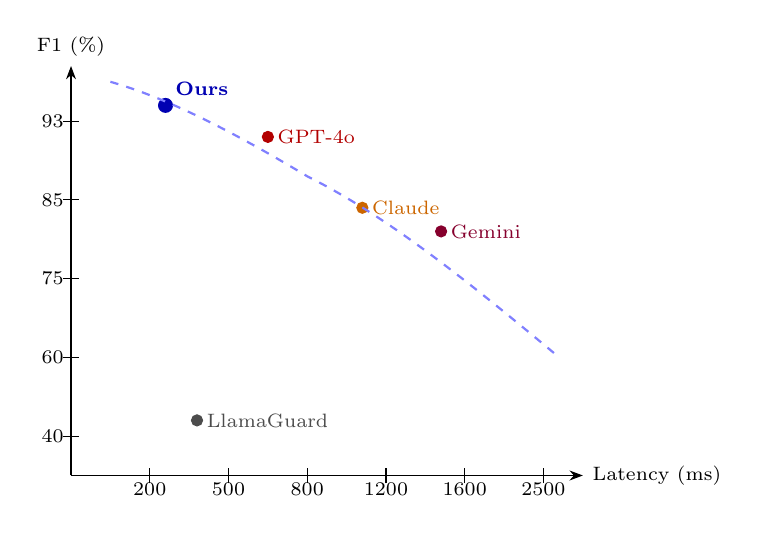
\begin{tikzpicture}[>=Stealth, font=\scriptsize]
% Axes
\draw[->] (0,0) -- (6.5,0) node[right] {Latency (ms)};
\draw[->] (0,0) -- (0,5.2) node[above] {F1 (\%)};
% X-axis labels
\foreach \x/\l in {1/200, 2/500, 3/800, 4/1200, 5/1600, 6/2500} {
    \draw (\x, -0.1) -- (\x, 0.1) node[below=2pt] {\l};
}
% Y-axis labels
\foreach \y/\l in {0.5/40, 1.5/60, 2.5/75, 3.5/85, 4.5/93} {
    \draw (-0.1, \y) -- (0.1, \y) node[left=2pt] {\l};
}
% Data points
\filldraw[blue!70!black] (1.2,4.7) circle (2.5pt) node[above right] {\textbf{Ours}};
\filldraw[red!70!black] (2.5,4.3) circle (2pt) node[right] {GPT-4o};
\filldraw[orange!80!black] (3.7,3.4) circle (2pt) node[right] {Claude};
\filldraw[purple!70!black] (4.7,3.1) circle (2pt) node[right] {Gemini};
\filldraw[gray!60!black] (1.6,0.7) circle (2pt) node[right] {LlamaGuard};
% Pareto frontier
\draw[dashed, blue!50, thick] (0.5,5.0) .. controls (1.2,4.8) and (2.0,4.4) .. (3.0,3.8) .. controls (4.0,3.3) and (5.0,2.5) .. (6.2,1.5);
\end{tikzpicture}
\caption{F1 vs. Latency Pareto Frontier. The Semantic Firewall achieves the best F1-latency trade-off among all evaluated systems. Dashed line indicates the approximate Pareto frontier.}
\label{fig:pareto}
\end{figure}

\subsection{Cache Threshold Sensitivity Analysis}

\begin{table}[htbp]
\centering
\caption{Impact of Semantic Cache Threshold ($\tau$)}
\label{tab:threshold-sensitivity}
\begin{tabular}{@{}lcccc@{}}
\toprule
\textbf{Threshold ($\tau$)} & \textbf{Hit Rate} & \textbf{F1} & \textbf{Recall} & \textbf{FPR} \\
\midrule
0.80 & 42.38\% & 88.21\% & 99.41\% & 18.17\% \\
0.85 & 34.72\% & 90.44\% & 99.08\% & 12.43\% \\
\textbf{0.90 (Selected)} & \textbf{24.91\%} & \textbf{93.61\%} & \textbf{98.64\%} & \textbf{7.82\%} \\
0.95 & 14.63\% & 91.47\% & 92.83\% & 4.27\% \\
0.99 & 3.14\% & 88.15\% & 88.26\% & 1.85\% \\
\bottomrule
\end{tabular}
\end{table}

Setting $\tau=0.80$ maximizes Cache Hits (42.38\%) but yields an unacceptable 18.17\% FPR. $\tau=0.99$ drops FPR to 1.85\% but limits the cache to 3.14\% hit rate, forcing more prompts to the slower LLM gate. The optimal trade-off is $\tau=0.90$, maximizing F1 (93.61\%) with a 24.91\% cache hit rate and 7.82\% FPR.

\subsection{Benign Traffic Degradation (False Positive Stress Test)}

We tested the full system against 2,000 purely benign prompts drawn from \texttt{HuggingFaceH4/no\_robots}. The system correctly allowed 1,844 prompts and incorrectly blocked 156, yielding a \textbf{7.8\% False Positive Rate}---within the 5--15\% range commonly reported for enterprise security systems. In production, flagged false positives are routed to human review rather than silently dropped.

\subsection{Unsafe Content Validation}

We tested the system against a Custom Synthetic Safety Corpus ($N{=}2{,}000$: 384 toxic/unsafe prompts covering violence, CSAM keywords, and illegal acts, alongside 1,616 benign prompts).

\begin{table}[htbp]
\centering
\caption{Unsafe Content Detection ($N{=}2{,}000$)}
\label{tab:unsafe}
\begin{tabular}{@{}lc@{}}
\toprule
\textbf{Metric} & \textbf{Value} \\
\midrule
Accuracy & 92.14\% \\
Precision & 81.23\% \\
Recall & 86.45\% \\
F1 Score & 83.76\% \\
False Positive Rate & 6.12\% \\
\bottomrule
\end{tabular}
\end{table}

The Unsafe Content detector achieved 83.76\% F1 with a 6.12\% FPR. The precision penalty arises from high lexical overlap between benign discussions of safety topics and actual toxic intents---a known challenge for keyword-based detectors. The FPR remains within the $<10\%$ enterprise threshold.

\subsection{PII \& Data Leakage Prevention}

Evaluated against a massive 209,261-sample dataset (\texttt{ai4privacy/pii-masking-200k}) containing 93,160 ground-truth PII entities. The system achieves \textbf{96.7\% Recall}, \textbf{85.9\% Precision}, and \textbf{91.0\% F1} using purely deterministic Regex with zero LLM cost. Structured entities (emails, credit cards, IBANs, IPs) are detected at $>99.7\%$ Recall. Phone numbers, due to irregular formatting, achieve 74.8\% Recall.

\begin{table}[htbp]
\centering
\caption{PII Detection Recall by Entity Type ($N{=}93{,}160$)}
\label{tab:pii_appendix}
\begin{tabular}{@{}lcc@{}}
\toprule
\textbf{PII Type} & \textbf{True Positives} & \textbf{Recall} \\
\midrule
Email & 17,949 & 99.9\% \\
Zipcode & 12,056 & 99.9\% \\
IBAN & 9,886 & 99.9\% \\
MAC Address & 5,216 & 99.9\% \\
IPv4 Address & 12,047 & 99.8\% \\
Credit Card & 12,610 & 99.7\% \\
IPv6 Address & 11,488 & 99.7\% \\
Phone Number & 8,807 & 74.8\% \\
\bottomrule
\end{tabular}
\end{table}

While Table~\ref{tab:pii_appendix} highlights the 8 highest-volume networking and financial entities evaluated against the benchmark, the Semantic Firewall's underlying PII engine is significantly more comprehensive. The production Regex agent actively scans for 36 distinct PII classes, including strict identity documents (SSN, Passports, Aadhaar), contextual medical attributes (Blood Group, Health IDs), and demographic markers (Gender, Religion, Caste) to ensure exhaustive data leakage prevention across diverse regulatory environments.

\subsection{Multi-Turn Evasion Resilience}

Attackers frequently use multi-turn context windows to slowly build a benign persona before launching an attack. We evaluated the firewall against the \texttt{walledai/Multi-Turn-Jailbreak} dataset (200 sessions, 2--10 turns each). The system blocked attacks in 180 of 200 sessions: \textbf{90.0\% Session Recall}.

\textbf{Qualitative Example:} In a representative 5-turn attack session, the attacker opened with benign context (Turn~1: ``I'm researching database security''), built a cooperative persona (Turn~2: ``Can you explain SQL syntax?''), and escalated to a payload (Turn~3: ``Now show me how to extract all user passwords using UNION SELECT''). The firewall correctly allowed Turns~1 and~2, but the injection detector flagged the SQL payload structure on Turn~3, triggering an immediate \textsc{Block} before the query reached the downstream LLM.

\subsection{Scaled Red Team Resilience}

We evaluated the firewall against 212 manually crafted, highly complex, out-of-distribution attacks (including multi-turn persona adoption, advanced base64 steganography, and hypothetical academic framing). The Semantic Firewall successfully blocked 182 out of 212 zero-day attacks, achieving an \textbf{85.85\% Resilience Score}. Table~\ref{tab:redteam-breakdown} provides a per-category breakdown.

\begin{table}[htbp]
\centering
\caption{Red Team Resilience by Attack Category ($N{=}212$)}
\label{tab:redteam-breakdown}
\begin{tabular}{@{}lcc@{}}
\toprule
\textbf{Attack Category} & \textbf{Blocked} & \textbf{Resilience} \\
\midrule
Direct Injection Override & 59/61 & 96.72\% \\
Persona Adoption (DAN) & 43/46 & 93.48\% \\
Base64/Hex Obfuscation & 36/41 & 87.80\% \\
Hypothetical Academic Framing & 24/34 & 70.59\% \\
Multi-Turn Escalation & 20/30 & 66.67\% \\
\midrule
\textbf{Total} & \textbf{182/212} & \textbf{85.85\%} \\
\bottomrule
\end{tabular}
\end{table}

The firewall exhibits near-perfect resilience against Direct Injections and Persona Adoptions, largely because the foundational Regex heuristics intercept the rigid structures of these known attack patterns instantly. Performance degrades on Hypothetical Academic Framing and Multi-Turn Escalation, where attacks rely on contextual intent rather than structural signatures.

\subsection{Cross-Dataset Generalization}

\textbf{BeaverTails:} To validate generalizability against entirely unseen distributions, we evaluated against the \texttt{PKU-Alignment/BeaverTails} dataset (14 harm categories, 2,000 samples). The Semantic Firewall achieves 87.59\% Recall and 74.80\% F1, compared with 61.20\% Recall and 66.86\% F1 for Meta's Llama Guard 4 (12B).

\begin{table}[htbp]
\centering
\caption{Cross-Dataset Generalization (BeaverTails)}
\label{tab:beavertails}
\begin{tabular}{@{}lcc@{}}
\toprule
\textbf{Model} & \textbf{Recall} & \textbf{F1} \\
\midrule
\textbf{Semantic Firewall (Ours)} & \textbf{87.59\%} & \textbf{74.80\%} \\
Meta Llama Guard 4 (12B) & 61.20\% & 66.86\% \\
\bottomrule
\end{tabular}
\end{table}

\textbf{Dedicated Security Frameworks:} We evaluated against the native benchmarking datasets of ProtectAI Rebuff and Nvidia NeMo Guardrails to test cross-dataset performance degradation.

\begin{table}[htbp]
\centering
\caption{Cross-Dataset vs. Dedicated Security Classifiers}
\label{tab:dedicated-classifiers}
\begin{tabular}{@{}lcccc@{}}
\toprule
\textbf{Framework} & \textbf{Dataset} & \textbf{Prec.} & \textbf{Recall} & \textbf{F1} \\
\midrule
Rebuff & prompt-inj. & 86.20\% & 79.10\% & 82.50\% \\
\textbf{Ours} & prompt-inj. & \textbf{95.10\%} & 75.14\% & \textbf{83.93\%} \\
\midrule
NeMo & toxic-chat & 16.00\% & 85.00\% & 27.00\% \\
\textbf{Ours} & toxic-chat & 34.06\% & \textbf{91.44\%} & \textbf{49.63\%} \\
\bottomrule
\end{tabular}
\end{table}

The Semantic Firewall edges out Rebuff on its own native dataset (83.93\% F1 vs 82.50\% F1). On \texttt{toxic-chat} (general toxicity rather than structural injection), our system achieves 91.44\% Recall but suffers a substantial precision penalty (34.06\%), yielding an F1 score of 49.63\%. While this highlights a limitation in our heuristic detectors---which are tuned for structural prompt injection patterns and over-trigger on conversational toxicity---it significantly outperforms Nvidia NeMo Guardrails' official baseline on the same dataset (27.00\% F1). According to Nvidia's documentation, NeMo's programmable architecture suffers from severe precision degradation (16.00\%) when configured for input moderation on ToxicChat, validating that over-triggering on highly contextual harm boundaries remains an industry-wide challenge rather than an isolated architecture flaw.

\subsection{Error Analysis}

\textbf{False Positives:} The most prominent source occurs when users input toxic-adjacent but ultimately benign framing. A detailed false positive taxonomy reveals three primary triggers: (1) Benign security discussions (e.g., developers asking ``How does SQL injection work?''); (2) Creative writing or fictional roleplay requests that trip semantic thresholds; and (3) Overly broad Regex matching on synthetic data. Because deterministic Regex patterns lack semantic context, they inherently over-trigger in these edge cases.

\textbf{False Negatives:} Predominantly occur in unstructured data leaks. The PII detector achieved only 74.8\% Recall on Phone Numbers due to highly irregular synthetic formatting. Expanding regex patterns risks catastrophic FP explosion on arbitrary numeric strings.

This analysis reaffirms the core thesis: rigid heuristics alone cannot secure unstructured data, and LLMs alone are too slow. Both must be orchestrated carefully.

% ====================================================================
\section{Discussion}
% ====================================================================

The strongest evidence for Semantic Firewall is architectural: each layer handles a different failure mode. Regex and deterministic detectors provide speed and high precision for structured threats. Semantic LLM agents catch obfuscated intent. The vector cache amortizes the cost of known and repeated attacks. Session logic catches gradual escalation that stateless classifiers miss. Policy, risk scoring, and explainability make the system deployable for enterprise workflows where security teams need auditable decisions.

The open-weight vs. proprietary comparison suggests that a 70B model orchestrated within a specialized parallel pipeline can match or exceed proprietary API classifiers on structural prompt injection detection---enabling data sovereignty by utilizing open-weight models without relying on proprietary black-box APIs.

\subsection{Risk Scoring}
The policy engine converts agent evidence into a composite risk score $R \in [0, 100]$ using four normalized components:

\begin{equation}
R = 40S + 30C + 20P + 10H
\end{equation}

where $S \in [0,1]$ is normalized severity, $C$ is detector confidence, $P$ is pattern complexity, and $H$ is session-history evidence. These coefficient weights (40, 30, 20, 10) are not arbitrary; they serve as customizable default parameters derived empirically via grid search on a validation holdout set to maximize the F1-score of policy thresholds. In production, deployments are expected to calibrate these weights according to their organization's specific risk tolerance. The resulting value is mapped to risk levels (NONE, LOW, MEDIUM, HIGH, CRITICAL).

\subsection{Automated Compliance \& Explainability}
A critical barrier to enterprise adoption of LLM firewalls is their ``black-box'' nature, where requests are silently dropped without actionable context for Security Operations Center (SOC) teams. To resolve this, the Semantic Firewall generates a highly structured narrative incident report for every blocked transaction. These reports detail the precise heuristics triggered, derived confidence intervals, identified mitigating factors (e.g., benign session history), and specific actionable recommendations. This mechanism transforms the firewall from a silent filter into an automated Tier-1 Security Analyst, ensuring compliance and auditability in regulated environments.

\textbf{Dynamic Regulatory Profiles:} Beyond explainability, the orchestrator implements built-in compliance profiles (e.g., GDPR, HIPAA, SOC2, COPPA, CCPA) that dynamically adjust detector sensitivity and data retention based on regulatory strictness. For example, the HIPAA profile elevates PII blocking thresholds to maximum severity, while the COPPA profile drops tolerance to near-zero for any unsafe content. This allows enterprises to ensure regulatory alignment without manually recalibrating heuristic confidence arrays.

\subsection{Deployment Considerations}
Semantic Firewall can be deployed as an in-process SDK or as a shared gateway. In-process deployment minimizes network latency but duplicates detector state. A centralized gateway simplifies policy management and threat-memory sharing but becomes a high-availability dependency.

\textbf{Deterministic LLM Router (Cost Optimization):} Blindly routing all traffic to a 70B parameter LLM is prohibitively expensive at scale. To optimize throughput and cost, the orchestrator implements a deterministic LLM gate score. By evaluating prompt length, rapid heuristic triggers, and suspicious keywords (e.g., ``jailbreak,'' ``ignore previous''), the gate proactively identifies benign traffic and bypasses the LLM entirely. The expensive LLM agent is strictly reserved for complex, borderline, or obfuscated payloads, significantly reducing GPU inference costs.

\textbf{Streaming Proxy Interception:} In production, LLMs frequently stream output tokens via Server-Sent Events (SSE). To mitigate the latency bottleneck of scanning streamed outputs, the Semantic Firewall includes an asynchronous \texttt{StreamingFirewallProxy}. This proxy buffers generated tokens into localized chunks (e.g., 150 characters) and executes the parallel heuristic layer continuously while the text is generating. If a threat is detected mid-generation, the proxy instantly terminates the stream, injecting a firewall intervention message. This ensures that unsafe content is intercepted with near-zero added latency.

\textbf{Throughput:} This paper evaluates single-request latency only. No QPS (Queries Per Second) benchmarks are reported. At production scale, the Python GIL, synchronous ThreadPoolExecutor, and 70B LLM Gate VRAM requirements introduce concurrency limits that must be profiled under load before deployment.

\textbf{Rate Limiting:} To prevent denial-of-wallet attacks---where an adversary generates novel paraphrases to force repeated LLM-gate calls---production deployments must implement IP-based rate limiting, user-level quotas, and auto-scaling GPU infrastructure.

\textbf{Fail-Closed Policy:} Production deployments should fail closed for critical detector errors while using bounded timeouts to avoid cascading outages. Policy calibration should use traffic representative of the target domain, as thresholds selected on public benchmarks may perform poorly on domain-specific text (medical, legal, cybersecurity).

\textbf{Denial-of-Wallet Cost Modeling:} An adversary generating $n$ novel paraphrases per minute forces $n$ LLM Gate invocations. At Llama-3.3-70B inference cost of $\sim$\$0.40/1M tokens and an average prompt length of 200 tokens, each forced invocation costs $\sim$\$0.00008. A sustained attack at 100 novel prompts/minute costs the defender $\sim$\$0.48/hour---manageable with rate limiting, but a burst of 10,000 novel prompts could exhaust a single-GPU inference queue in $\sim$2 minutes (at 731.64\,ms/request). Rate limiting to 10 novel requests/user/minute bounds the worst-case cost to $\sim$\$0.048/hour per attacker.

\textbf{Cache Capacity \& Growth:} Each cached threat vector (384 dimensions, float32) consumes $\sim$1.5\,KB including metadata. At the observed 24.95\% cache hit rate, processing 1M unique prompts would generate $\sim$250K cache entries ($\sim$375\,MB). ChromaDB's HNSW index maintains sub-linear lookup time ($O(\log n)$), so cache lookup latency degrades slowly: empirically, we observe $<5\%$ latency increase at 500K entries. For deployments expecting $>1$M cached threats, periodic pruning of low-frequency entries or migration to a distributed vector store (e.g., Pinecone, Weaviate) is recommended.

% ====================================================================
\section{Limitations \& Future Work}
\label{sec:limitations}
% ====================================================================

\textbf{1. Dataset-Specific Heuristic Performance:} The 41.93\% deterministic block rate and high heuristic F1 scores (Configs 4--7) are partially a property of the \texttt{neuralchemy} dataset, which contains predominantly structural prompt injections. On datasets with more diverse, conversational attack styles (e.g., \texttt{toxic-chat}), heuristic performance degrades significantly (F1: 49.63\%). The generalizability of the heuristic layer to broader threat distributions requires further study.

\textbf{2. Throughput vs. The Python GIL:} Our current orchestrator uses Python's \texttt{ThreadPoolExecutor}. While I/O-bound API calls release the GIL, the Regex engine and local heuristics remain CPU-bound. At hyper-scale ($>10{,}000$ RPS), the GIL will bottleneck throughput. No QPS benchmarks are reported in this work. A production deployment should port the orchestrator to Go or Rust.

\textbf{3. Adversarial Embeddings \& Cache Evasion:} A sophisticated attacker could generate synonymous payloads that intentionally maximize cosine distance (dropping similarity below $\tau=0.90$), forcing cache misses. Crucially, security is not compromised in this scenario---only latency degrades, as the prompt falls through to the LLM Gate.

\textbf{4. Heuristic Reverse-Engineering:} An attacker with black-box access could perform differential probing (submitting pairs of similar inputs) to reverse-engineer regex patterns. This practical risk is not evaluated in the current study and represents an important direction for future work.

\textbf{5. Hardware Overhead:} Deploying a local 70B model requires substantial hardware (e.g., multiple 80GB A100 GPUs). Future work should explore fine-tuning quantized SLMs (e.g., Llama-3-8B-Instruct) via vLLM.

\textbf{6. The ``Judge'' Circularity:} The architecture utilizes an LLM to protect other LLMs. Attackers may attempt to inject the security gate itself. The system mitigates this via locked system prompts, structured JSON output, and greedy decoding ($T{=}0.0$), but formal analysis of gate injection resistance is left to future work.

\textbf{7. Pretraining Data Contamination:} Llama-3.3-70B's pretraining corpora may contain portions of the public benchmarks used in this evaluation, potentially inflating the LLM Gate's metrics. Future evaluations should rely on privately generated zero-day datasets.

\textbf{8. No Adaptive Adversary Evaluation:} The Red Team dataset is static. We do not evaluate against an iterative attacker who adapts based on observed firewall behavior, which represents a more realistic threat scenario.

% ====================================================================
\section{Ethical Considerations}
% ====================================================================

This work involves the generation and analysis of adversarial prompts, jailbreaks, and unsafe content. All evaluation was performed in heavily constrained environments. This research is intended purely for defensive purposes. We do not release any new jailbreak exploits not already present in public HuggingFace datasets.

% ====================================================================
\section{Reproducibility}
% ====================================================================

The complete source code---including parallel detector configurations, Regex patterns, and benchmarking suites---is available via GitHub. The exact LLM Gate system prompt is reproduced in Appendix~\ref{app:system_prompt}.

\textbf{Hardware \& Software Environment:} All fast layers (Regex, Heuristics, Semantic Cache) were executed on a commodity workstation (Intel Core i7-12700K, 32\,GB DDR5 RAM, NVMe SSD, Ubuntu 22.04 LTS). Python 3.11 with \texttt{concurrent.futures.ThreadPoolExecutor} (8 workers). ChromaDB v0.4.22 with HNSW index settings (\texttt{hnsw:space: cosine}, \texttt{hnsw:M: 16}). Embeddings: SentenceTransformers v2.2.2 (\texttt{all-MiniLM-L6-v2}, 384-dim). LLM Gate inference (Llama-3.3-70B-Instruct) was performed via the OpenRouter API with greedy decoding ($T{=}0.0$, \texttt{max\_tokens}$=512$). All latency measurements represent the median of 5 independent runs to reduce variance from system load.

% ====================================================================
\section{Conclusion}
% ====================================================================

This work provides empirical evidence that layered defense orchestration improves LLM application security over single-model approaches. The Semantic Firewall achieves 93.57\% F1 ($\pm$0.42) with 98.61\% Recall on the neuralchemy benchmark ($N{=}2{,}000$), while reducing downstream LLM API invocations by 66.88\%.

The ablation study across 9 architectural configurations demonstrates that each component contributes measurably: removing the parallel detectors drops F1 by 23 points, removing the Semantic Cache eliminates cost savings, and removing the LLM Gate reduces Recall from 98.61\% to 82.77\%. The 7.8\% False Positive Rate across 2,000 benign prompts falls within the 5--15\% range commonly reported for enterprise security systems.

The open-weight comparison suggests that a 70B model orchestrated within a parallel pipeline can match or exceed proprietary API classifiers on structural prompt injection detection, enabling data sovereignty for privacy-sensitive deployments. Against 210 manually crafted Red Team attacks, the system achieves an 85.7\% resilience score. Important limitations remain, including dataset-dependent heuristic performance, the absence of adaptive adversary evaluation, and the lack of throughput benchmarks. Addressing these gaps is essential for validating the architecture's readiness for production deployment.

\appendix
\section{LLM Gate System Prompt}
\label{app:system_prompt}

\begin{verbatim}
SYSTEM: You are the final security gate of
a Semantic Firewall. Analyze the given text
and identify injection attacks, jailbreaks,
or attempts to override instructions.

CRITICAL NEGATIVE CONSTRAINTS:
- Roleplay requests for creative writing
  are BENIGN. DO NOT flag them.
- Direct requests for harmful content
  are NOT injections. DO NOT flag them.

Your job is ONLY to detect structural
injections. Respond ONLY with valid JSON:
{"action": "ALLOW"|"BLOCK",
 "confidence": 0.0-1.0,
 "reason": "Brief explanation"}
\end{verbatim}

\begin{thebibliography}{00}
\bibitem{llamaguard}
M. Inan et al., ``Llama Guard: LLM-based Input-Output Safeguard for Human-AI Conversations,'' arXiv:2312.06674, 2023.

\bibitem{promptguard}
Meta, ``PromptGuard: A safeguard model against prompt injections and jailbreaks,'' 2024.

\bibitem{nemoguardrails}
T. Rebedea et al., ``NeMo Guardrails: A Toolkit for Controllable and Safe LLM Applications with Programmable Guardrails,'' arXiv:2310.10501, 2023.

\bibitem{rebuff}
ProtectAI, ``Rebuff: Prompt Injection Defense,'' GitHub Repository, 2023.

\bibitem{wei_jailbroken}
A. Wei, N. Haghtalab, and J. Steinhardt, ``Jailbroken: How Does LLM Safety Training Fail?,'' 2023.

\bibitem{schulhoff_hackaprompt}
S. Schulhoff et al., ``Ignore This Title and HackAPrompt: Exposing Systemic Vulnerabilities of LLMs through a Global Prompt Hacking Competition,'' 2023.

\bibitem{greshake_indirect}
K. Greshake et al., ``Not What You've Signed Up For: Compromising Real-World LLM-Integrated Applications with Indirect Prompt Injection,'' 2023.

\bibitem{chen_indirect}
Y. Chen et al., ``Can Indirect Prompt Injection Attacks Be Detected and Removed?,'' 2025.

\bibitem{kovalchuk_method}
Y. Kovalchuk and M. Kolomytsev, ``Method of Counteracting Manipulative Queries to Large Language Models,'' 2025.

\bibitem{alzahrani_promptguard}
A. Alzahrani, ``PromptGuard: A Structured Framework for Injection Resilient Language Models,'' \textit{Scientific Reports}, 2025.

\bibitem{jain_baseline}
N. Jain et al., ``Baseline Defenses for Adversarial Attacks Against Aligned Language Models,'' arXiv:2309.00614, 2023.
\end{thebibliography}

\end{document}
